\section{Results}\label{sec:results}
Using \fidanka we fit pairs of Population A + E isochrones to the HUGS data for
NGC 2808. Each pair of isochrones is allowed to vary in distance modulus,
reddening, relative helium mass fraction (A/E), and age. Any population pairs which vary by more than 1\% in distance modulus or B-V color excess are rejected. The $\chi^{2}$
distribution for the isochrone pairs is shown in Figure {\color{red}[FIGURE]}.
The best fit isochrones are shown in Figure \ref{fig:BestFitResults} and optimized
parameters for these are presented in Table {\color{red}[TABLE]}.

{\color{red} Need to make the chi2 dist plot still. Have all these values but need to figure out best way to visualize it}

\begin{figure}
  \centering
  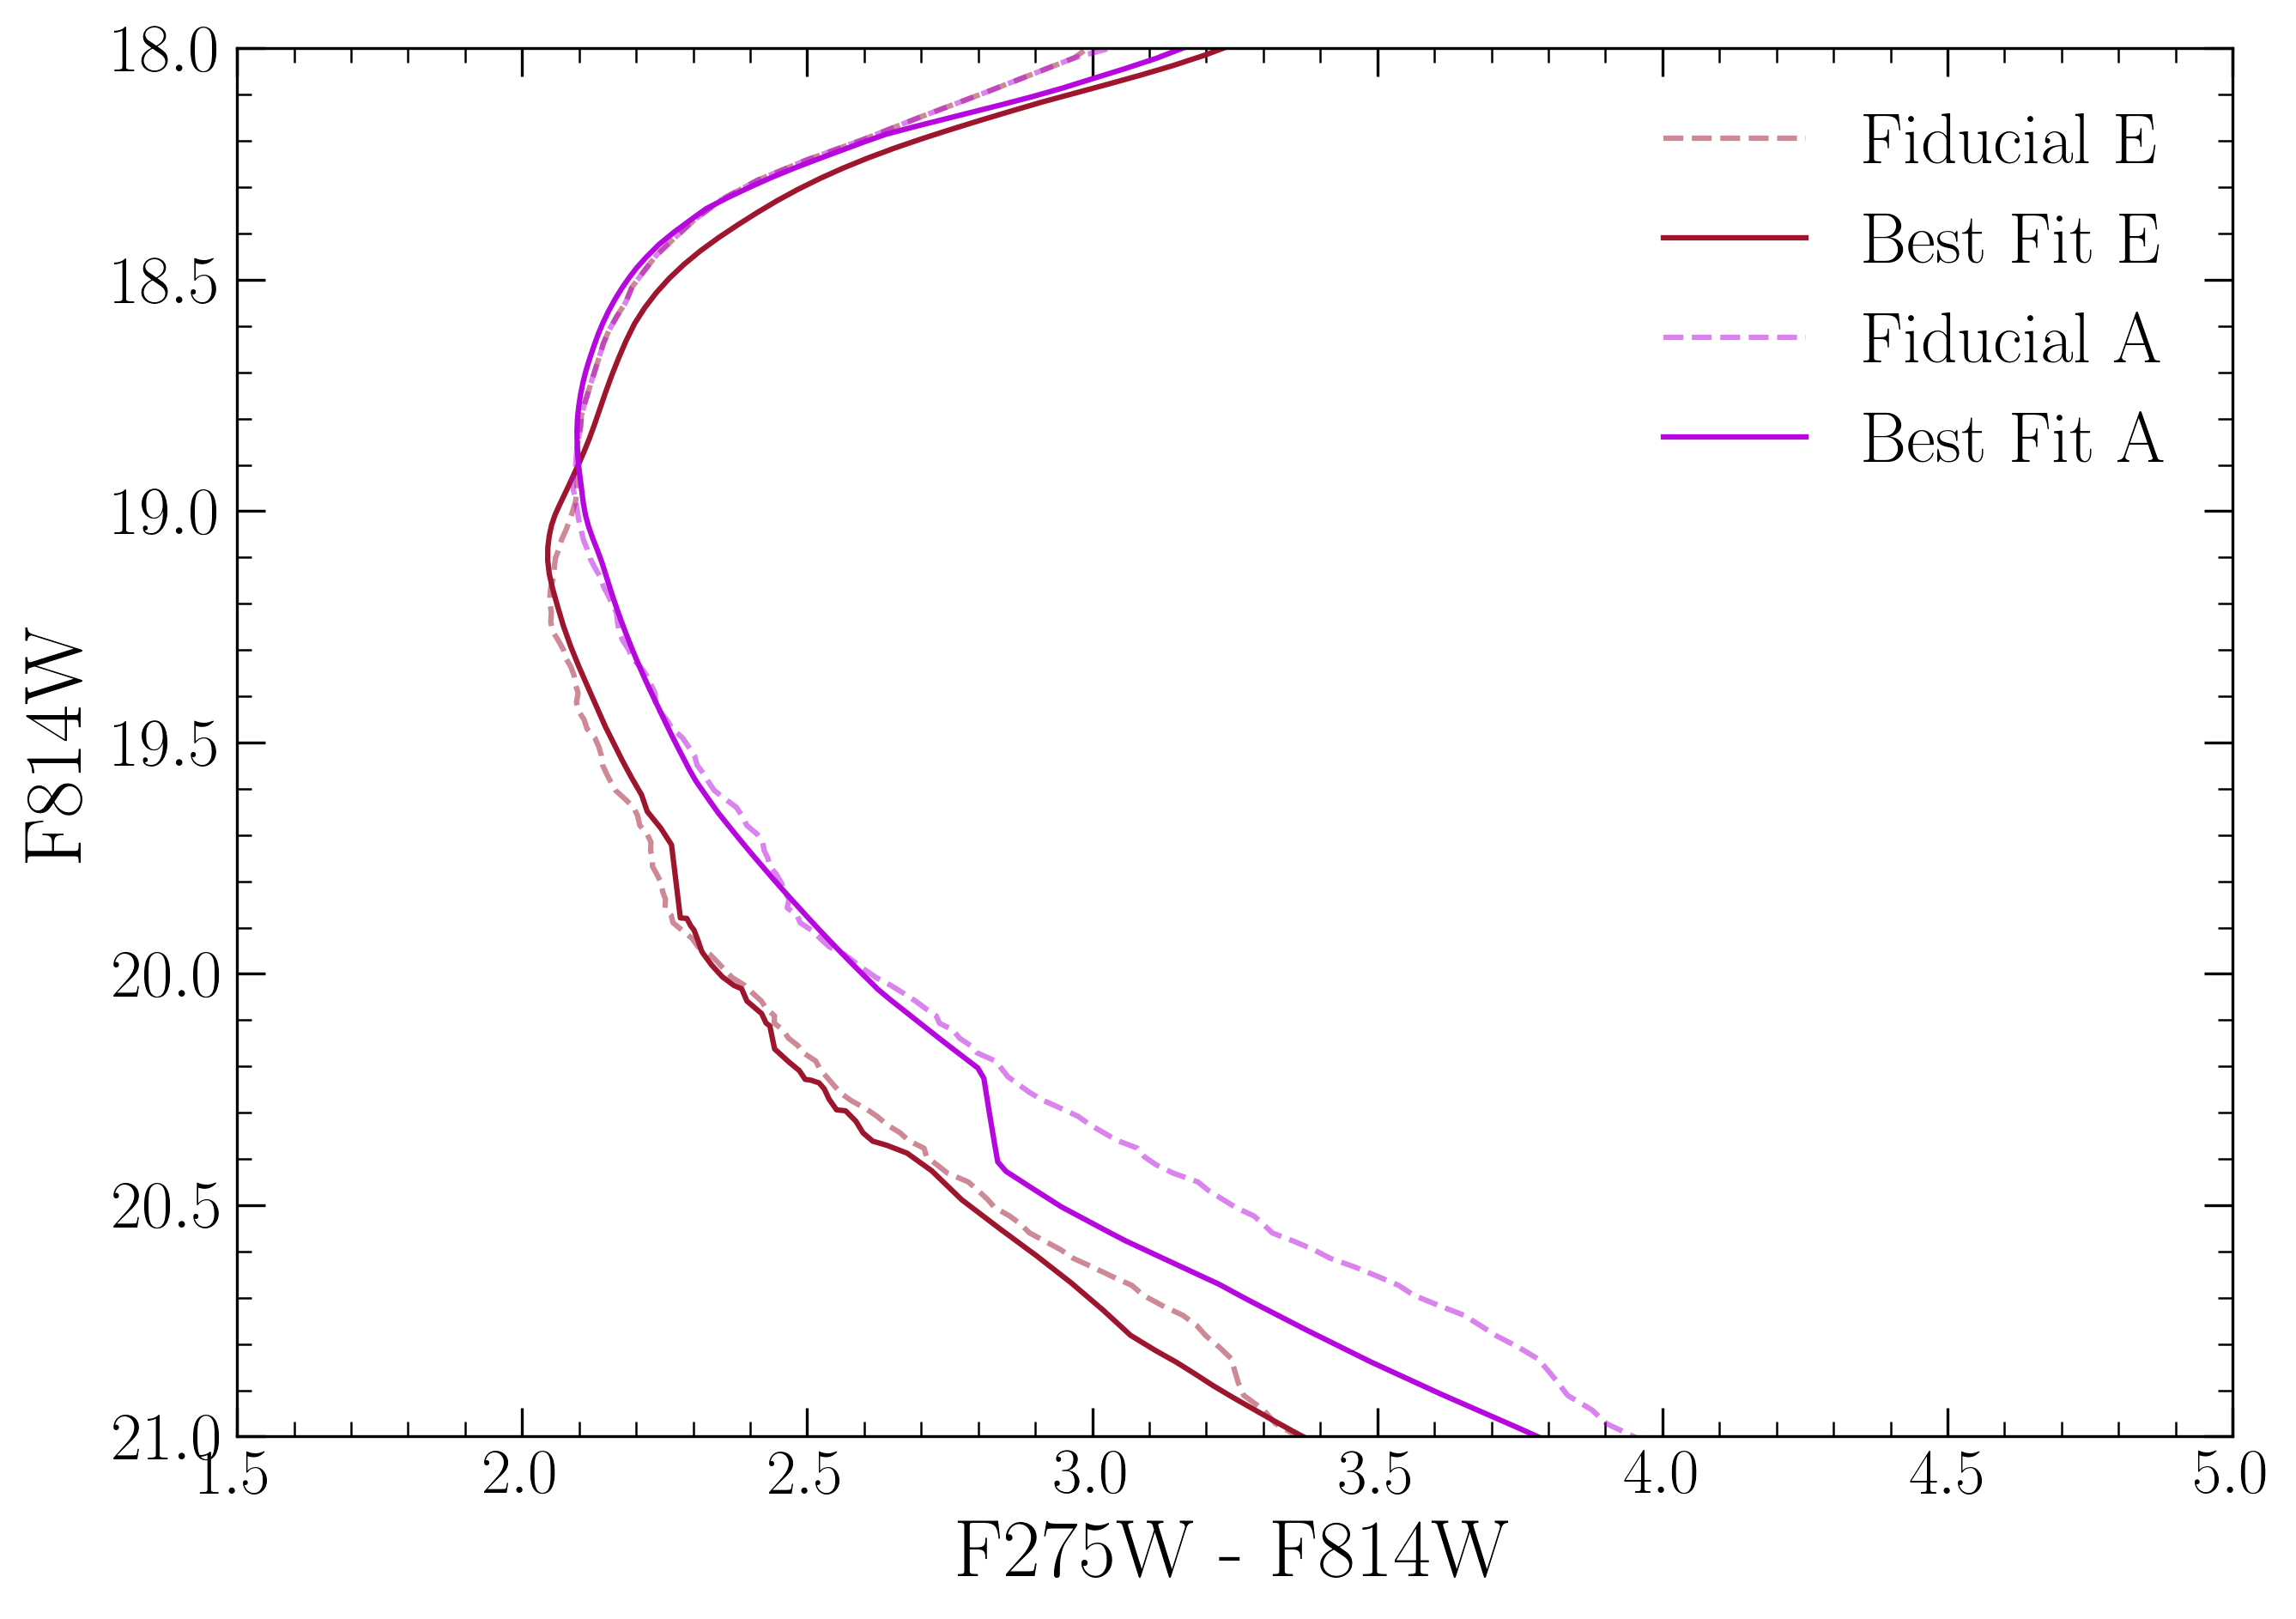
\includegraphics[width=0.45\textwidth]{src/figures/BestFit.png}
  \label{fig:BestFitResults}
  \caption{Best fit isochrone results for NGC 2808.}
\end{figure}

{\color{blue} Currently are still seeing a discontinutiy in the isochrobne below the MSTO. This must be addressed before submission.}
